\subsubsection*{例1: 棒グラフを1つ描画する}

\verb|dat1.csv|ファイルの\verb|Age|を構成要素項目に、
\verb|Population|を構成量項目として棒グラフを1つ描画する。

\begin{Verbatim}[baselinestretch=0.7,frame=single]
$ more dat1.csv
Age,Population
10,310504
20,552339
30,259034.5555
40,0450818
50,1231572
60,1215966
70,641667
$ mbar.rb i=dat1.csv v=Population f=Age o=result1.html
#END# mbar.rb i=dat1.csv v=Population f=Age o=result1.html;
\end{Verbatim}

以下の棒グラフが描画される。

ブラウザで表示した棒グラフにマウスカーソルを置くと、
構成要素項目とその構成量がポップアップで表示される。
グラフはマウスによるドラッグ操作で移動することができ、
またマウスのスクロール操作によって拡大縮小もできる。

\begin{flushleft}
\fbox{
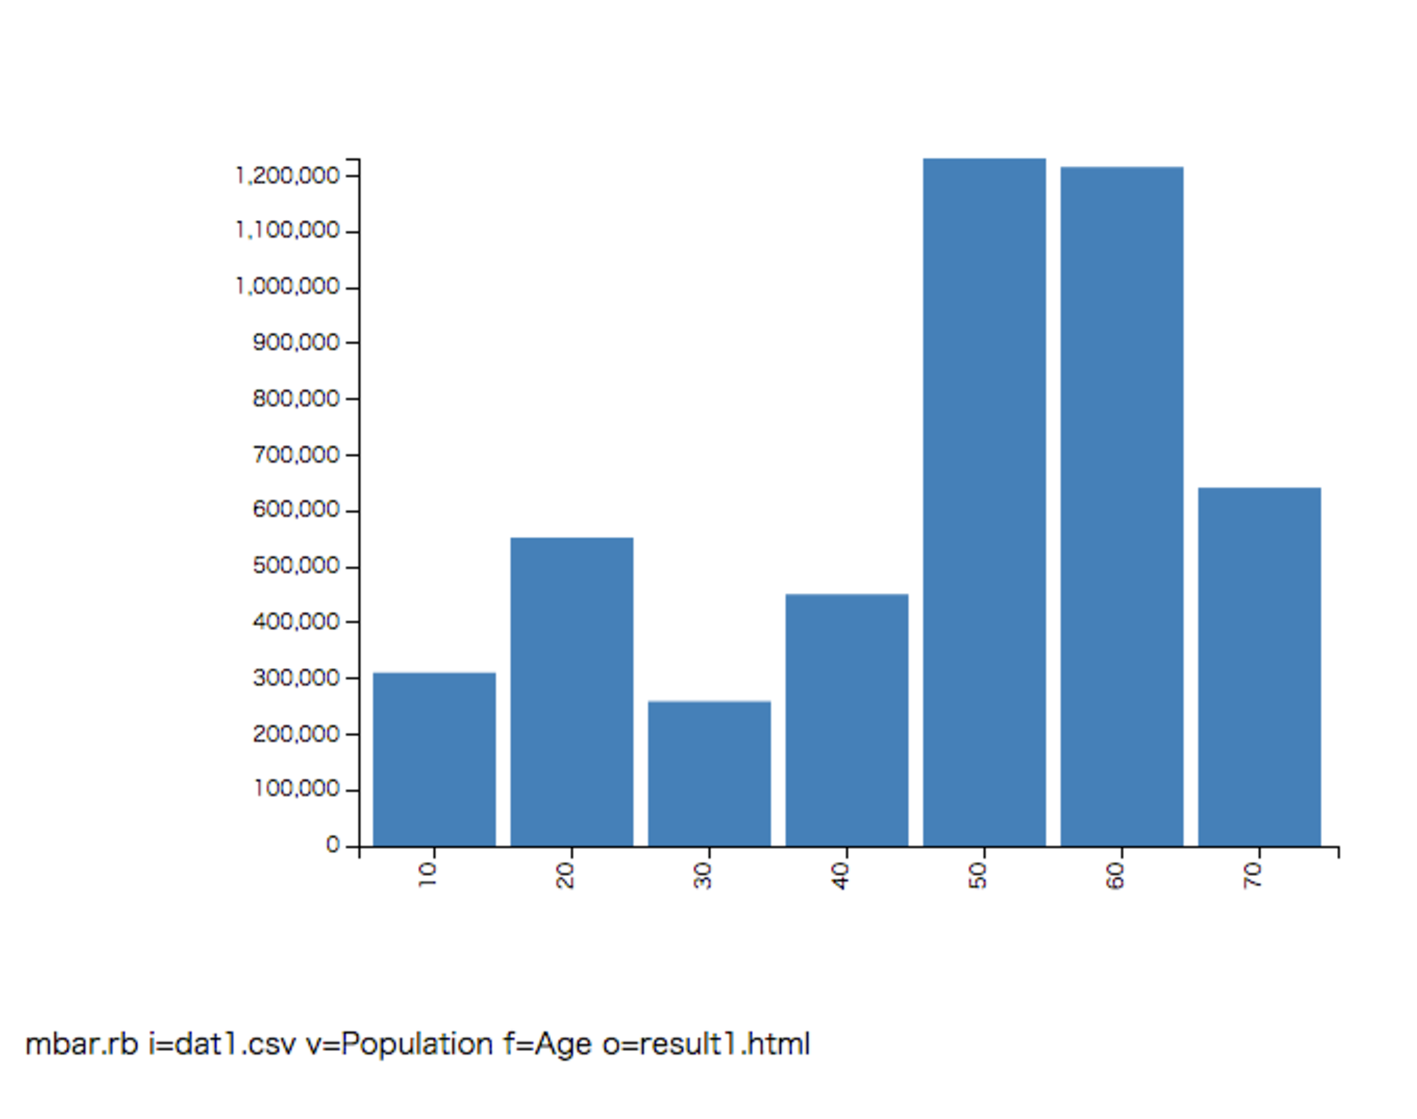
\includegraphics[scale=0.5]{figure/mbar1.eps}
}
\end{flushleft}

\subsubsection*{例2: 1次元の棒グラフ行列を描画する}

\verb|dat2.csv|ファイルの\verb|Age|を構成要素項目に、
\verb|Population|を構成量項目として棒グラフを描画する。
\verb|k=|パラメータに\verb|Pref|項目を指定しているので、
\verb|Pref|項目の値をx軸(横方向)に展開した1次元の棒グラフ行列が描画される。
\verb|title=|パラメータでグラフのタイトルも指定している。

\begin{Verbatim}[baselinestretch=0.7,frame=single]
$ more dat2.csv
Pref,Age,Population
奈良,10,310504
奈良,20,552339
奈良,30,259034
奈良,40,450818
奈良,50,1231572
奈良,60,1215966
奈良,70,641667
北海道,10,310504
北海道,20,252339
北海道,30,859034
北海道,40,150818
北海道,50,9231572
北海道,60,4215966
北海道,70,341667
$ mbar.rb i=dat2.csv k=Pref v=Population f=Age o=result2.html
 title=奈良と北海道の年代ごとの人口
#END# mbar.rb i=dat2.csv k=Pref v=Population f=Age o=result2.html
title=奈良と北海道の年代ごとの人口;
\end{Verbatim}

以下の棒グラフ行列が描画される。

\begin{flushleft}
\fbox{
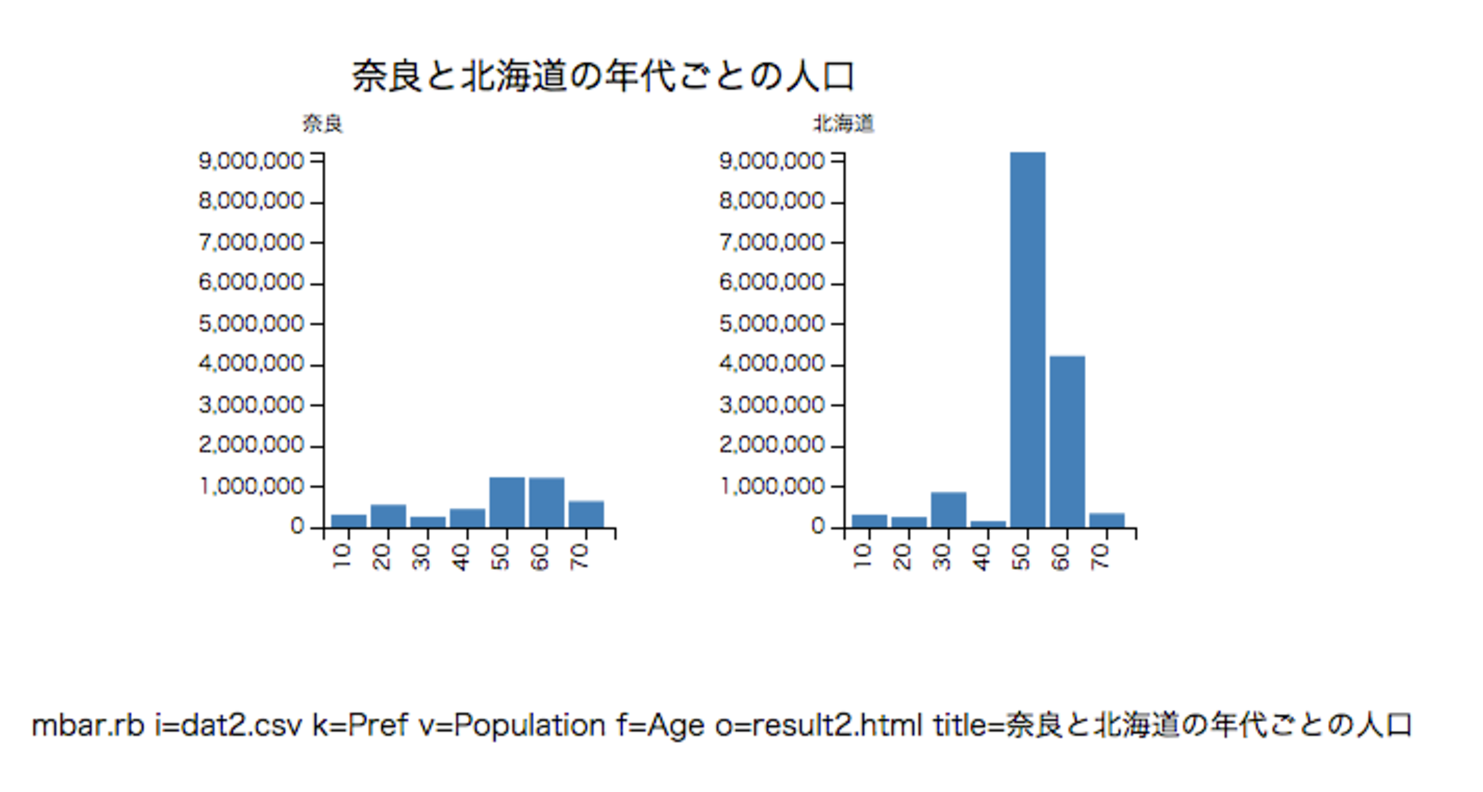
\includegraphics[scale=0.5]{figure/mbar2.eps}
}
\end{flushleft}

\subsubsection*{例3: 2次元の棒グラフ行列を描画する}

\verb|dat3.csv|ファイルの\verb|テーマパーク名|を構成要素項目、
\verb|Number|を構成量項目とし、\verb|width=|に幅200、\verb|height=|に高さ150を指定して、
棒グラフを描画する。
\verb|k=|パラメータに\verb|Gender|と\verb|Age|項目を指定しているので、
\verb|Gender|項目の値をx軸(横方向)に、
\verb|Age|項目の値をy軸(縦方向)に展開した2次元の棒グラフ行列が描画される。

\begin{noautoxspacing}
\begin{Verbatim}[baselinestretch=0.7,frame=single]
$ more dat3.csv
Gender,Age,テーマパーク名,Number
男性,30,デズニ,100
男性,30,UFJ,59
男性,30,梅屋敷,180
男性,40,デズニ,200
男性,40,UFJ,3
男性,40,梅屋敷,10
男性,50,デズニ,110
男性,50,UFJ,40
女性,30,梅屋敷,100
女性,30,デズニ,80
女性,30,UFJ,200
女性,40,デズニ,90
女性,40,UFJ,80
女性,40,梅屋敷,120
女性,50,デズニ,99
女性,50,UFJ,80
女性,50,梅屋敷,110
$ mbar.rb i=dat3.csv k=Gender,Age v=Number f=テーマパーク名 o=result3.html
 title=性別と年代ごとのテーマパーク訪問回 width=200 height=150
#END# ./bin/mbar.rb i=dat3.csv k=Gender,Age v=Number f=テーマパーク名 o=result3.html 
title=性別と年代ごとのテーマパーク訪問回 width=200 height=150;
\end{Verbatim}
\end{noautoxspacing}

以下の棒グラフ行列が描画される。

\begin{flushleft}
\fbox{
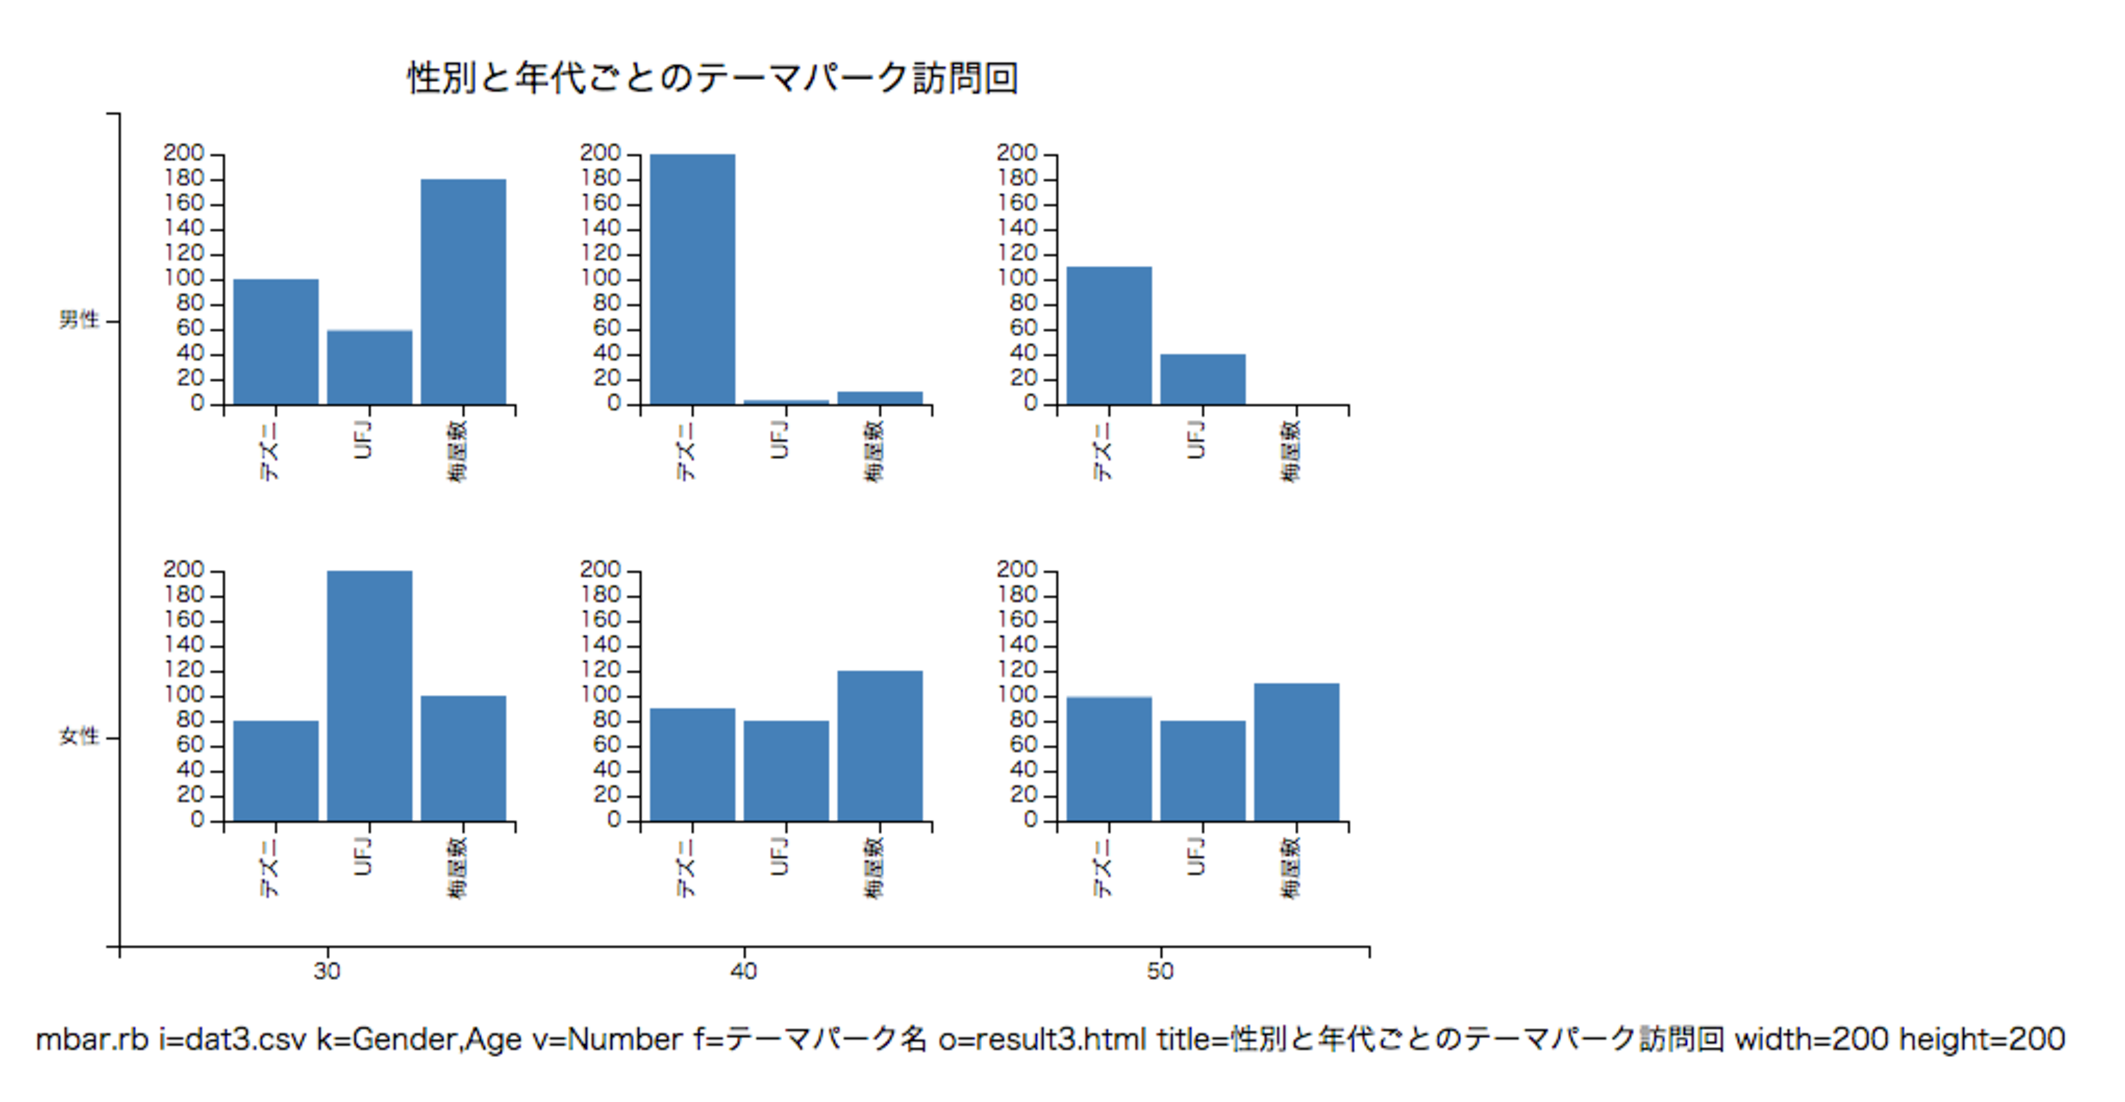
\includegraphics[scale=0.5]{figure/mbar3.eps}
}
\end{flushleft}
